

\documentclass[color=usenames,dvipsnames]{beamer}

\usepackage[adobefonts,noindent]{ctex} %中文支持
\setCJKmainfont{SimSun}

\mode<presentation> {

\usetheme{Madrid}
\usecolortheme{lily}
\useoutertheme{infolines}

}


\usepackage{booktabs} 
\usepackage{tikz}


\newcommand{\red}[1]{\textcolor{red}{#1}}
\newcommand{\brown}[1]{\textcolor{brown}{#1}}
\newcommand{\green}[1]{\textcolor{green}{#1}}
\newcommand{\blue}[1]{\textcolor{blue}{#1}}
\newcommand{\cyan}[1]{\textcolor{cyan}{#1}}

% 可缩放版block
\newenvironment<>{varblock}[2][.9\textwidth]{%
    \setlength{\textwidth}{#1}
    \begin{actionenv}#3%
        \def\insertblocktitle{#2}%
        \par%
        \usebeamertemplate{block begin}}
    {\par%
        \usebeamertemplate{block end}%
    \end{actionenv}}


% Thin fonts
\usepackage{cmbright}
\usepackage[T1]{fontenc}

\definecolor{dark_grey}{gray}{0.5}
\setbeamercolor{normal text}{fg=dark_grey,bg=white}
\setbeamertemplate{navigation symbols}{}

\setbeamercolor*{palette primary}{fg=gray!100,bg=gray!10}
\setbeamercolor*{palette quaternary}{fg=gray!100,bg=gray!10}
\setbeamercolor*{palette secondary}{fg=gray!100,bg=gray!20}
\setbeamercolor*{palette tertiary}{fg=gray!100,bg=gray!10}
\setbeamercolor*{navigation symbols}{fg=white,bg=white}
\usefonttheme{default}


\setbeamertemplate{blocks}[rounded][shadow=false]
\setbeamercolor{block title}{bg=gray!10}
\setbeamercolor{block body}{fg=gray,bg=gray!10}
%\setbeamercolor{frametitle}{fg=}

\setbeamertemplate{frametitle}[default][center]

\setbeamertemplate{itemize items}[default]
\setbeamertemplate{enumerate items}[default]

\newcommand{\F}{\mathbb{F}}


\title[KB+Desc Embed]{Representation Learning of Knowledge Graphs with Entity Descriptions}
\subtitle{AAAI 2016}
\author[韩喆]{谢若冰, 刘知远, 贾珈 , Huanbo Luan, 孙茂松}
\institute[ICSTWIP]{Tsinghua University}
\date[20160311]{}
\begin{document}


\begin{frame}
  \titlepage
\end{frame}

% Uncomment these lines for an automatically generated outline.
%\begin{frame}{Outline}
%  \tableofcontents
%\end{frame}

\begin{frame}{outline}
 \begin{itemize}
  \item 作者简介
  \item 论文简介
  \item 相关工作:transXXX, socher.NTN
  \item 模型
  \item 实验内容、效果
  \item \textbf{手动}对比
 \end{itemize}
\end{frame}

\begin{frame}{作者简介}\footnotesize
  \begin{columns}
   \column{0.3\hsize}
     \begin{block}{}
   \begin{center}
    \begin{figure}
     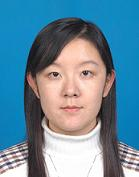
\includegraphics[width=0.45\hsize]{pic/jiajia.jpg}
     \caption{\href{http://media.cs.tsinghua.edu.cn/cn/jiajia}{贾珈}}
    \end{figure}
   \end{center}
   \begin{itemize}
    \item 情感计算、语音交互...
   \end{itemize}
     \end{block}

   \column{0.3\hsize}
   \begin{block}{}\centering
    \textbf{谢若冰}
   \end{block}
     \begin{block}{}
   \begin{center}
    \begin{figure}
     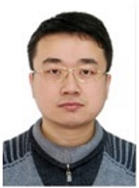
\includegraphics[width=0.45\hsize]{pic/liuzhiyuan.jpg}
     \caption{\href{http://nlp.csai.tsinghua.edu.cn/~lzy/}{刘知远}}
    \end{figure}
   \end{center}
   \begin{itemize}
    \item KG,语义计算,“社会计算”...
   \end{itemize}
     \end{block}
   \begin{block}{}\centering
    \textbf{Huanbo Luan}
   \end{block}
     
   \column{0.3\hsize}
     \begin{block}{}
   \begin{center}
    \begin{figure}
     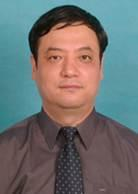
\includegraphics[width=0.45\hsize]{pic/sunmaosong.jpg}
     \caption{\href{http://nlp.csai.tsinghua.edu.cn/site2/index.php/people?id=16}{孙茂松}}
    \end{figure}
   \end{center}
   \begin{itemize}
    \item 计算语言学,汉语切词...
   \end{itemize}
     \end{block}
  \end{columns}

\end{frame}


\frame{
  \begin{columns}[c]
   \column{.15\hsize}
   \column{.7\hsize}
   \begin{block}{}
    \centering \Large 论文简介  \\ 
   \end{block}
   \column{.15\hsize}
  \end{columns}
}

\frame{
  \frametitle{论文简介}
  \begin{enumerate}\small
   \item 以前的词向量从KB/KG学习,但是KG是非常稀疏的
  \pause
   \item KB中对应三元组少的、没有三元组对应(zero-shot)的实体的词向量很不好
  \pause
   \item 实体可能没有三元组,但一般都有维基百科页面正文
   \item 我要把KB和自然语言text结合,放在一起训练,生成一个\textbf{更好}的词向量
  \end{enumerate}
  
  \pause
\begin{center}
            \begin{minipage}{6cm}
   \begin{varblock}[6cm]{什么叫\red{更好}?}
    比transE好就可以叫更好了 \\ 
   \end{varblock}
            \end{minipage}
        \end{center}
    \begin{center}
     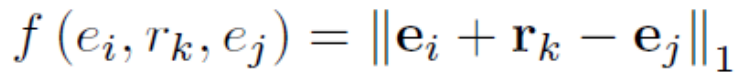
\includegraphics[width=0.5\hsize]{pic/transE1.png} \\
     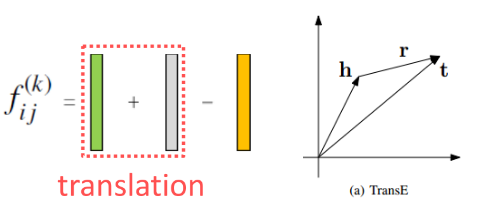
\includegraphics[width=0.5\hsize]{pic/transE2.png} \\
    \end{center}
}


\frame{
  \begin{columns}[c]
   \column{.15\hsize}
   \column{.7\hsize}
   \begin{block}{}
    \centering \Large 相关工作  \\ 
   \end{block}
   \column{.15\hsize}
  \end{columns}
}

\frame{
  \frametitle{相关工作-1}
  \begin{columns}[c]
   \column{0.27\hsize}
  \begin{block}{transE,transR, PTransE}
     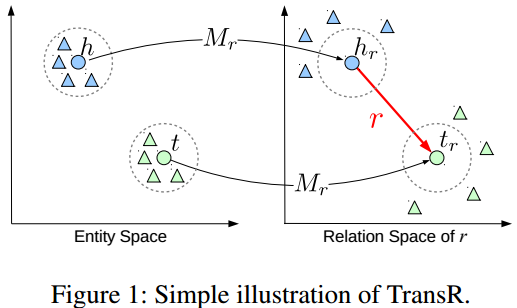
\includegraphics[width=0.95\hsize]{pic/transR.png}\\ 
      \begin{figure}
     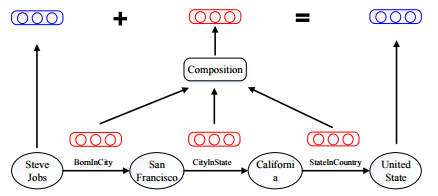
\includegraphics[width=0.85\hsize]{pic/PtransE.png}
       \caption{PTransE}
      \end{figure}
%     \begin{columns}[c]
%      \column{0.45\hsize}
%      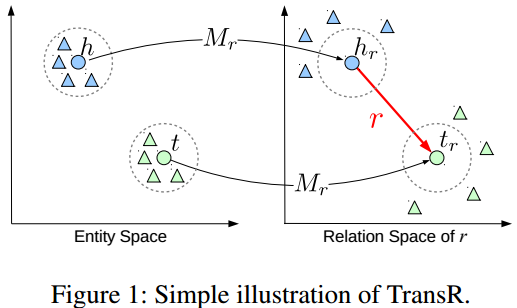
\includegraphics[width=0.65\hsize]{pic/transR.png} 
% 
%      \column{0.45\hsize}
%       \begin{figure}
%      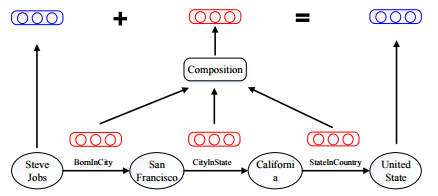
\includegraphics[width=0.55\hsize]{pic/PtransE.png}
%        \caption{PTransE}
%       \end{figure}
% 
%     \end{columns}
  \end{block}
  
  \column{0.7\hsize}
  \begin{block}{NTN (neural tensor network, socher)}\small
  使用组成当前短语的单词的词向量的平均值能一定程度代表当前单词的词向量 \\
     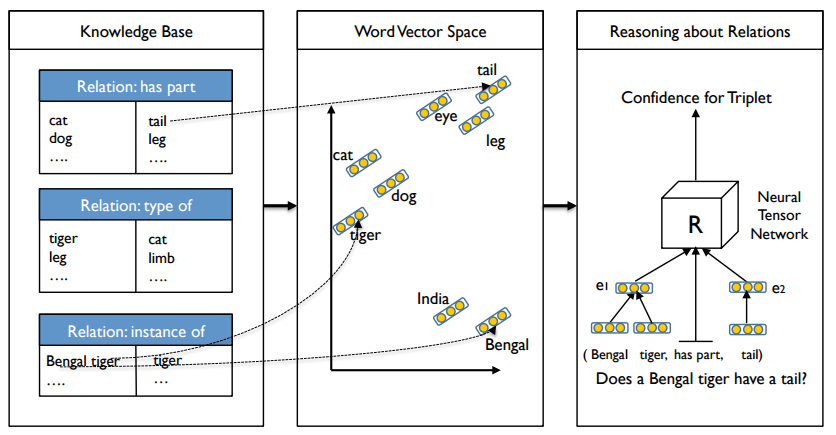
\includegraphics[width=0.99\hsize]{pic/NTN.png} \\
  \end{block}
  \end{columns}
}


\frame{
  \frametitle{相关工作-2}
  \begin{block}{KB+WikipediaAnchor}
   利用WikipediaAnchor([[迈克尔·乔丹|乔丹]]?) 来增大单词之间的联系
  \end{block}
  \begin{block}{KB+Description}
    \begin{itemize}
     \item 和上一个同一个作者
     \item 构造一个复杂的目标函数:KB的目标(h+r-t 小)+文本相似(文本中距离近的单词距离小)+description相似(一个实体的文本中的单词和他距离进)
     \item \blue{本文作者认为:}上述模型没有考虑文本顺序,模型没有考虑/无法避免文本的歧义
    \end{itemize}
  \end{block}
}

\frame{
  \begin{columns}[c]
   \column{.15\hsize}
   \column{.7\hsize}
   \begin{block}{}
    \centering \Large 模型  \\ 
   \end{block}
   \column{.15\hsize}
  \end{columns}
}

\frame{
  \frametitle{模型}
  \begin{itemize}
   \item $(h,r,t)\in T, h,t\in E, r\in R$
   \item 每个实体($h$或$t$)同时训练2个向量$h_s$(从\red{triple}中学习的向量), $h_d$(从\red{正文}中学习的向量)
   \item 目标函数 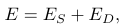
\includegraphics[height=0.05\hsize]{pic/lossFunc1.png} 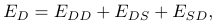
\includegraphics[height=0.05\hsize]{pic/lossFunc2.png}
    \begin{itemize}
     \item 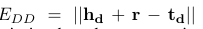
\includegraphics[height=0.045\hsize]{pic/EDD.png}
     \item 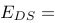
\includegraphics[height=0.045\hsize]{pic/EDS.png}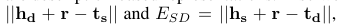
\includegraphics[height=0.045\hsize]{pic/ESD.png}
    \end{itemize}
  \end{itemize}
}

\frame{
  \frametitle{模型-Encoder}
  \begin{itemize}
   \item 2种Encoder生成从正文中学习的\red{文本向量}:CBOW、CNN
  \end{itemize}
  
  \begin{columns}
   \column{0.42\hsize}
   \begin{block}{CBOW}
   \begin{enumerate}\footnotesize
    \item 根据tf-idf值,在每个实体页面中取最重要的\textbf{20}个单词作为他的文本特征
    \item 将这20个单词的词向量的平均值作为该实体的文本向量的值
   \end{enumerate}
   \centering 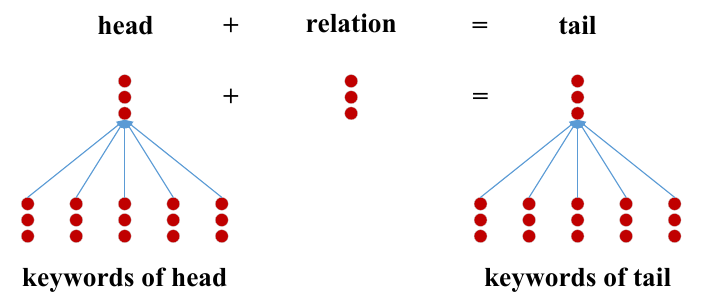
\includegraphics[width=0.95\hsize]{pic/CBOW.png} 
   \end{block}

   \column{0.55\hsize}
    \begin{block}{CNN}
     \begin{enumerate}\footnotesize
      \item (1->2).1 对将连续的\textbf{2}个单词的词向量拼接得到一个长的词向量$x_i'$
      \item (1->2).2 卷一下: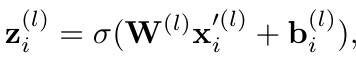
\includegraphics[width=0.3\hsize]{pic/zi.png} 
      \item (2->3) max-pooling:  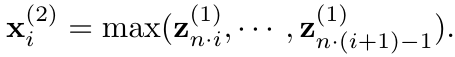
\includegraphics[width=0.45\hsize]{pic/maxpooling.png} 
      \item (3->4) 卷一下:同$z_i^{(1)}$,得到$z_i^{(2)}$
      \item (4->5) mean-pooling: 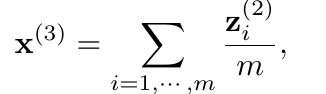
\includegraphics[width=0.25\hsize]{pic/meanpooling.png} 
     \end{enumerate}
   \centering 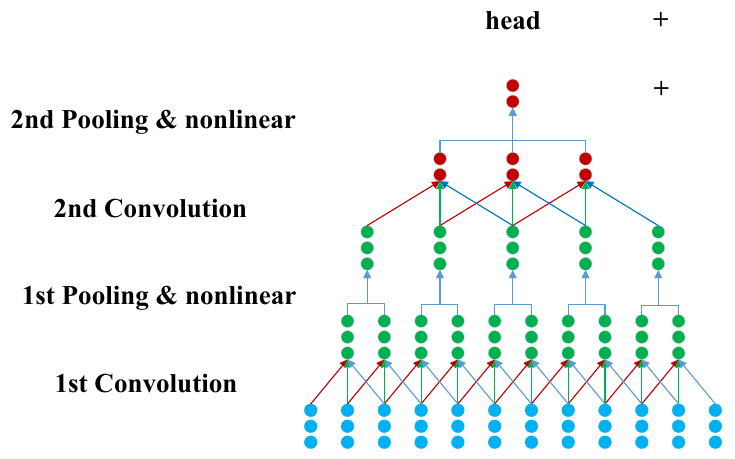
\includegraphics[width=0.7\hsize]{pic/CNN.png} 
    \end{block}
  \end{columns}
}

\frame{
  \frametitle{模型-训练}
  \begin{block}{目标函数}\centering
   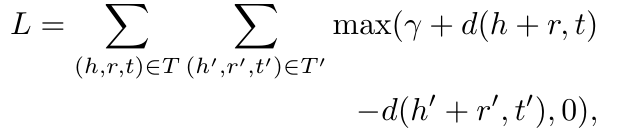
\includegraphics[width=0.4\hsize]{pic/lf1.png} 负样本:	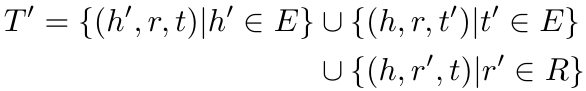
\includegraphics[width=0.4\hsize]{pic/lf2.png} 
  \end{block}

  \begin{itemize}
   \item 距离函数$d$为L1范式(绝对值相加,又称曼哈顿距离)
   \item 负样本中的新实体向量既可以使用triple向量,也可以使用文本向量
   \item 待训练的参数集合为
\includegraphics[width=0.25\hsize]{pic/para.png}:文本向量、2个卷积矩阵、实体向量、关系向量
   \item $X$由word2vec在维基百科上先跑好,$E,R$可以随机初始化,也可以使用transE的结果
  \end{itemize}
}



\frame{
  \begin{columns}[c]
   \column{.15\hsize}
   \column{.7\hsize}
   \begin{block}{}
    \centering \Large 实验  \\ 
   \end{block}
   \column{.15\hsize}
  \end{columns}
}

\frame{
  \frametitle{实验-数据集、参数}
  \begin{columns}
   \column{0.5\hsize}\centering
   \begin{figure}
   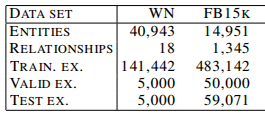
\includegraphics[width=0.6\hsize]{pic/fb15k.png}
   \caption{原始的FB15k}
   \end{figure}

   \column{0.5\hsize}\centering
   \begin{figure}
   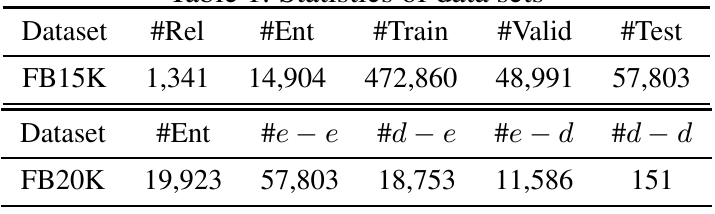
\includegraphics[width=0.9\hsize]{pic/fb15kX.png}
   \caption{本实验的数据集}
   \end{figure}
  \end{columns}

  \begin{itemize}
   \item 作者去除了正文过短的实体(<3个单词)
   \item 为了验证Zero-shot,作者将fb15k扩充成fb20k:
    \begin{itemize}
     \item 从freebase中随机选和fb15k有triple关系的新点加进来,最后把新点和集合中其他实体的triple边加进来
    \end{itemize}
   \item 参数:学习率$\lambda=0.001$ margin:$\gamma=1$ 卷积初始合并$k=2$个连续单词 词向量$n=100$维, $n_w=100,n_f=100$
  \end{itemize}

}

\frame{
  \frametitle{实验-KBC-1}
  \begin{columns}
   \column{0.5\hsize}
  \begin{block}{}
   补全三元组,\red{预测实体}:$(h,r,t)$:给定$r,t$,求$h$;或者给定$h,r$,求$t$
  \end{block}
   \column{0.5\hsize}
  \begin{center}
   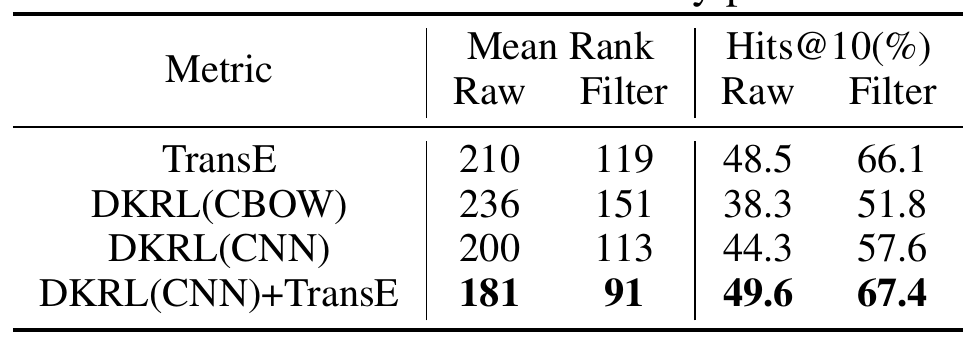
\includegraphics[width=0.95\hsize]{pic/expKBC.png}
  \end{center}
  \end{columns}

  \begin{itemize}\small
   \item filter 指的是把预测结果中在训练集、测试集中出现的三元组删掉之后的效果
    \begin{itemize}\footnotesize
     \item 理论上在训练集中出现的三元组不会在测试集中出现,不可能是答案
    \end{itemize}
   \item transE原论文提供的HIT@10数据是$34.9, 47.1$
    \begin{itemize}\footnotesize
     \item 作者强调他自己实现了transE,比原论文效果好(实验结果没问题)
     \item 结论说自己的方法比transE有明显提升
     \pause
     \item 有点自相矛盾
    \end{itemize}
  \end{itemize}
}

\frame{
  \frametitle{实验-KBC-2}
  \begin{columns}
   \column{0.5\hsize}
  \begin{block}{}
   补全三元组,\blue{预测关系}:$(h,r,t)$:给定$h,t$,求$r$
  \end{block}
   \column{0.5\hsize}
  \begin{center}
   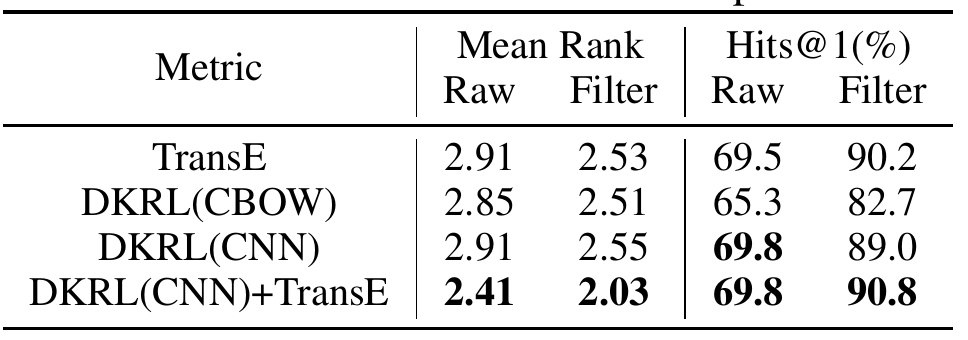
\includegraphics[width=0.95\hsize]{pic/expKBC2.png}
  \end{center}
  \end{columns}
}


\frame{
  \frametitle{实验-分类}
  \begin{enumerate}
   \item 取FB15K中实体的所有类别并统计频率,取出现频率最高的50个作为分类的候选
  \end{enumerate}
  
  \begin{center}
   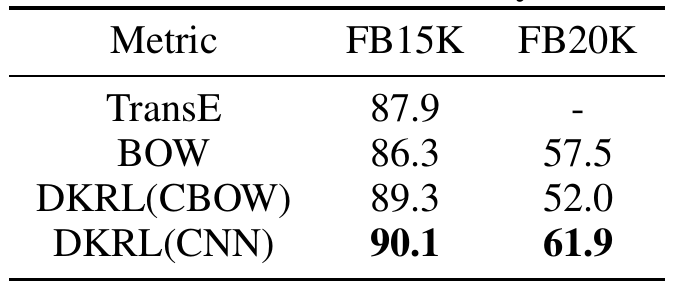
\includegraphics[width=0.49\hsize]{pic/expClass.png}
  \end{center}
  
  \begin{itemize}
   \item BOW:词袋模型,一个one-hot的超大vector,长度为词典大小
   \item 文本信息对于预测类别有相对明显的提升
  \end{itemize}
}


\frame{
  \frametitle{实验-zero-shot}
  \begin{itemize}\small
   \item 如果测试集中的实体在训练集中没有出现,则不可能训练出词向量,更不可能找到答案
   \item 在FB20K上看看本文效果(FB15K的测试集中大多数实体都出现过了)
   \item 使用FB15K的训练集,测试集改成FB20K多的那5K个实体引入的新三元组
  \end{itemize}
  
  \only<1>{
  \begin{block}{1.预测实体}
  \begin{center}
   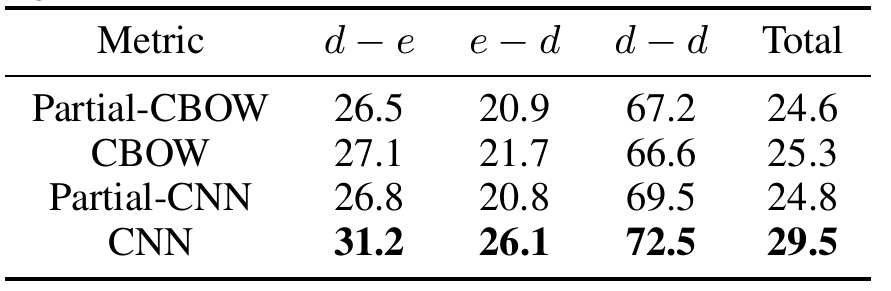
\includegraphics[width=0.5\hsize]{pic/expZero.png}
  \end{center}
  \begin{itemize}
   \item $d-e$ 表示head是新的实体,tail是原来FB15K训练集中的实体
   \item  Partial-XX 表示测试数据的时候在训练集中出现的实体用triple向量表示;否则,所有数据都用文本向量表示
  \end{itemize}
  \end{block}
  }
  \only<2>{
  \begin{block}{1.预测\red{关系}}
  \begin{center}
   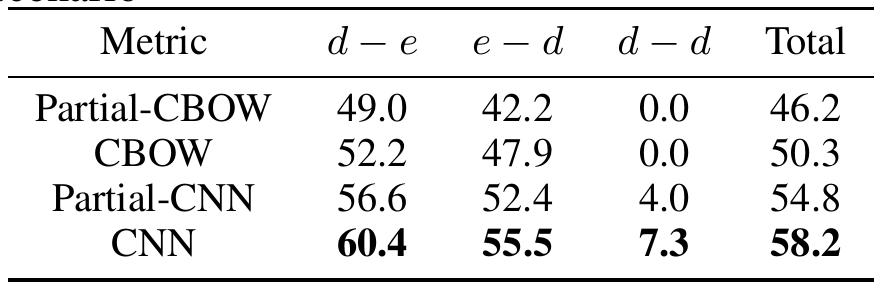
\includegraphics[width=0.5\hsize]{pic/expZeroRel.png}
  \end{center}
  \end{block}
  }
}


\frame{
  \begin{columns}[c]
   \column{.15\hsize}
   \column{.7\hsize}
   \begin{block}{}
    \centering \Large \textbf{手工}对比  \\ 
   \end{block}
   \column{.15\hsize}
  \end{columns}
}

\frame{
  \frametitle{手工对比}
  \begin{itemize}
   \item 原始的文章到zero-shot实验之后就结束了,开始总结
   \item 没有对比
  \end{itemize}
  
  \begin{block}{Aligning knowledge and text embeddings by entity descriptions}
   \begin{itemize}\footnotesize
    \item EMNLP 2015
    \item 构造一个复杂的目标函数:KB的目标(h+r-t 小)+文本相似(文本中距离近的单词距离小)+description相似(一个实体的文本中的单词和他距离进)
   \end{itemize}
  \end{block}
  \begin{block}{Representing Text for Joint Embedding of Text and Knowledge Bases}
   \begin{itemize}
    \item EMNLP 2015
    \item 用CNN encode 文本中的d-path
   \end{itemize}
  \end{block}
}

\frame{
  \frametitle{手工对比-Aligning knowledge and text embeddings by entity descriptions}
  \begin{itemize}
   \item 中山大学+微软
   \item 目标函数3方面: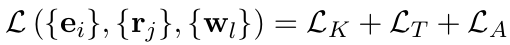
\includegraphics[width=0.35\hsize]{pic/exp1lf.png}
    \begin{itemize}\footnotesize
     \item KB的优化目标(h+r-t 小)+文本相似(文本中距离近的单词距离小)+description相似(一个实体的文本中的单词和他距离进)
     \item 以第一方面为例: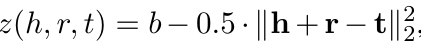
\includegraphics[width=0.35\hsize]{pic/exp1p2.png} \\ 
     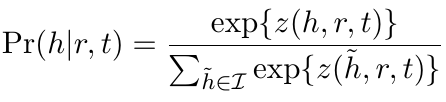
\includegraphics[width=0.35\hsize]{pic/exp1p1.png}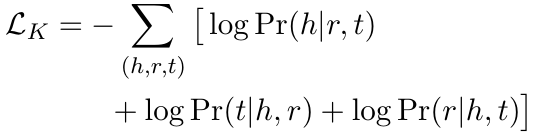
\includegraphics[width=0.35\hsize]{pic/exp1p3.png}
    \end{itemize}
    \item 对数据没有做过清洗
  \end{itemize}
  \only<1>{
  \begin{columns}
   \column{0.5\hsize}\centering
   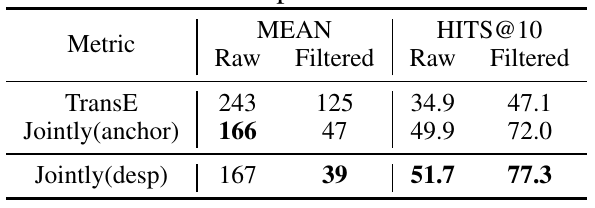
\includegraphics[width=0.85\hsize]{pic/exp1p4.png}
   \column{0.5\hsize}\centering
   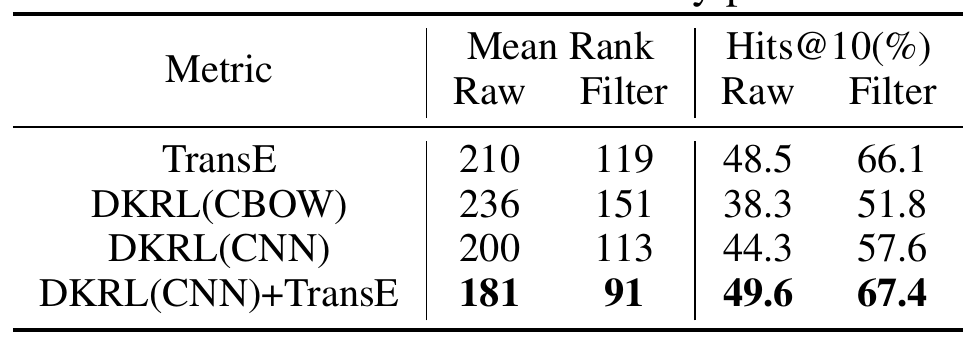
\includegraphics[width=0.85\hsize]{pic/expKBC.png}
  \end{columns}
  }
  \only<2>{
    \begin{itemize}
     \item 优点:效果好
     \item 缺点:归一化的概率计算复杂度大?
    \end{itemize}
  }

}

\frame{
  \frametitle{手工对比-Representing Text for Joint Embedding of Text and Knowledge Bases}
  \begin{itemize}
   \item Stanford+微软
   \item 不同于transE,提出E模型,DISTMULT模型来衡量三元组的可靠性
   \item 作者提取文本中的依存关系作为relation和entity的关联关系来训练relation向量
   
  \end{itemize}

  \only<1>{
  \begin{columns}
   \column{0.35\hsize}
   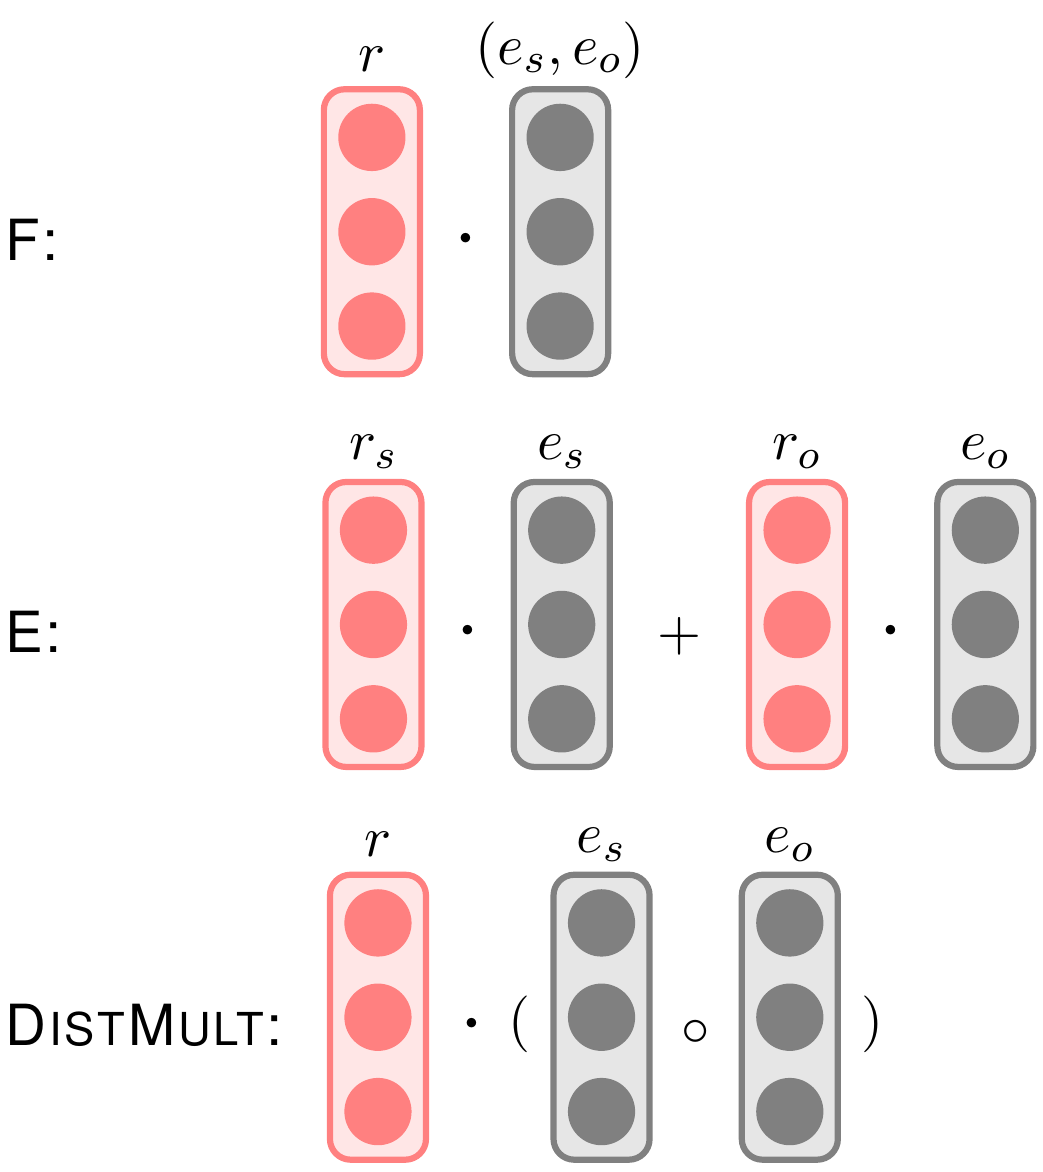
\includegraphics[width=0.95\hsize]{pic/models.png}
   
   \column{0.65\hsize}
   \begin{block}{E模型}
   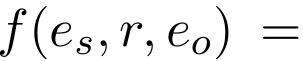
\includegraphics[width=0.35\hsize]{pic/emodel0.png}
   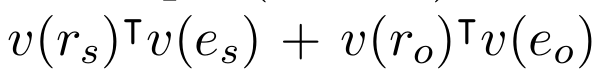
\includegraphics[width=0.5\hsize]{pic/emodel1.png}
   \end{block}
   \begin{block}{DISTMULT模型}
   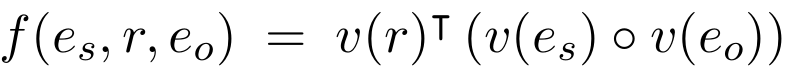
\includegraphics[width=0.95\hsize]{pic/fmodel.png}
   \end{block}
  \end{columns}
  }
  \only<2>{
  \begin{columns}
   \column{0.5\hsize}\centering
   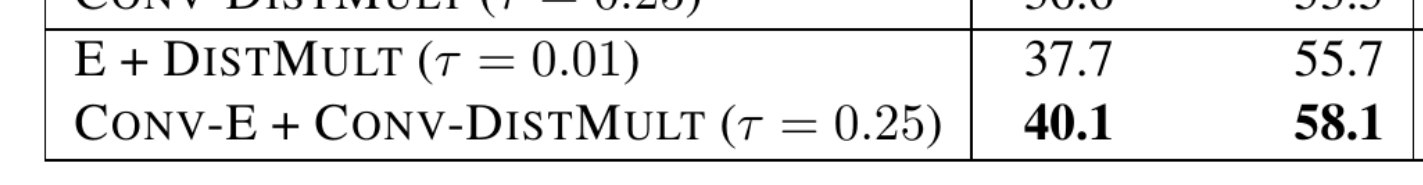
\includegraphics[width=0.85\hsize]{pic/exp2p1.png}
   \column{0.5\hsize}\centering
   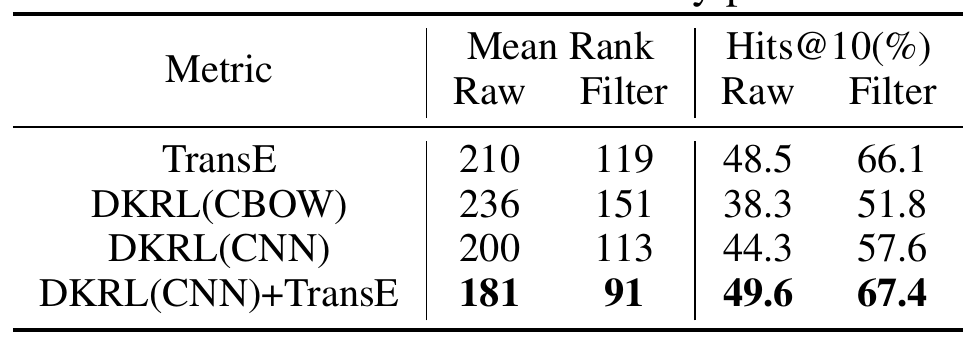
\includegraphics[width=0.85\hsize]{pic/expKBC.png}
  \end{columns}
  \begin{itemize}
   \item 这篇文章作者使用FB15K-237,更小/好的一个FB15K的子集
   \item 最后的效果并不比本文好
   \item TransE 其实已经是一个很好的模型了(?)
  \end{itemize}
  }
}

\frame{
  \frametitle{总结}
  \begin{itemize}
   \item text + KB 训练词向量,有提升,但很依赖怎么从文本中提取信息
    \begin{itemize}
     \item CNN 模型一般有小量提升,CBOW模型一般没有提升
     \item 怎么表示text 中的信息很重要
    \end{itemize}
   \item TransE模型已经很好了,工程使用应该够?
  \end{itemize}
}

\frame{
  \begin{columns}[c]
   \column{.2\hsize}
   \column{.6\hsize}
   \begin{block}{}
   \vspace{0.4cm}
    \centering \Large 问题?  \\ 
   \vspace{0.4cm}
   \end{block}
   \column{.2\hsize}
  \end{columns}
}
\end{document} 